\documentclass[aspectratio=43]{beamer}

\usetheme{simple}

\usepackage{lmodern}
\usepackage[scale=2]{ccicons}
\usepackage{hyperref}
\usepackage[inkscapeformat=png]{svg}

\usepackage[utf8]{inputenc} % No olvides utilizar UTF8, especialmente si tu presentación está en castellano


\def\edicion{XXXV} % Edición de las jornadas
\def\fecha{Abril 2023} % Fecha de las jornadas

\title{NixOS} % Modifica el título de la presentación a tu gusto
\subtitle{Linux dentro de 10 años} % Incluye un subtítulo si lo ves necesario, o bórralo
\author{Manuel Palenzuela Merino} % Cambia el autor de la presentación
\twitter{github.com/Baitinq} % Pon tu Twitter o déjalo en blanco

% Esto no lo cambies
\institute{\edicion \ Jornadas Técnicas del GUL}
\date{\fecha}


% Página principal (no tocar)
\titlegraphic{img/logo1.png}

\begin{document}

{
    \setbeamertemplate{footline}{}
    \begin{frame}
        \titlepage
    \end{frame}
}
\addtocounter{framenumber}{-1}

\setwatermark{
\includegraphics[height=8cm]{img/logo1.png}} % Marca de agua (opcional)

\section{Distribuciones de Linux "tradicionales"}
\subsection{Problemas}
\section{Que es Nix?}
\section{Nix (Lenguaje)}
\subsection{Derivaciones}
\section{Nixpkgs}
\section{Nix (Package Manager)}
\section{NixOS}
\subsection{Highlights}
\subsection{Configuraciones}
\section{El futuro de Linux}
\subsection{Mas informacion}
\section{Preguntas}

% ------------------------------------------------------------------------------------------
% La presentación empieza aquí. La primera diapositiva puede dejarse tal cual o sustituirse.
% ------------------------------------------------------------------------------------------

\begin{frame}
    \frametitle{Antes de empezar}
    \begin{enumerate}
        \item{Podeis preguntar dudas en cualquier momento}
        \item{Cuantas mas preguntas mejor :))}
        \item{Tambien se aceptan sugerencias durante la charla (mas alto, explicar algo mas a fondo, etc)}
        \item{\href{https://github.com/Baitinq/nixos-presentation}{https://github.com/Baitinq/nixos-presentation}}
    \end{enumerate}
\end{frame}

\begin{frame}
    \frametitle{Tabla de contenidos} % Puedes ponerle un título más chulo a la diapositiva con el índice de contenidos o dejar éste
    \tableofcontents % Para poblar la tabla de contenidos debes utilizar \section y \subsection apropiadamente (ver demo)
\end{frame}

\begin{frame}
    \frametitle{Distribuciones de Linux "tradicionales"}
        \begin{columns}
    \column{0.4\textwidth}
        Ej:
        \begin{itemize}
            \item{Arch Linux}
            \item{Debian}
            \item{Fedora}
            \item{Ubuntu}
        \end{itemize}
    \column{0.4\textwidth}
        Que son:
        \begin{enumerate}
            \item Package manager
            \item Repositorios
            \item Filesystem structure
            \item Etc?
        \end{enumerate}
    \end{columns}
\end{frame}

% TODO: Do sections in table of contents
\begin{frame}
    \frametitle{Problemas de distros "tradicionales"}
    \begin{itemize}
        \item Actualizaciones/cambios de configuración modifican destructivamente el estado del sistema (sobrescribiendo archivos en secuencia -\> \textbf{inconsistencia temporal})
        \item Diferentes versiones de un binario
        \item Conflictos de paquetes
        \item No hay rollbacks
        \item No hay gestión de la configuración (dotfiles)
        \item\textbf{NO HAY DETERMINISMO}
    \end{itemize}
\end{frame}

\begin{frame}
    \frametitle{Que es Nix?}
    
    \begin{enumerate}[I]
    \item{\href{https://nix.dev/tutorials/nix-language}{Nix (lenguaje)}}
    \item{\href{https://github.com/NixOS/nixpkgs}{Nixpkgs}}
    \item{\href{https://github.com/NixOS/nix}{Nix (package manager)}}
    \end{enumerate}

\end{frame}

\begin{frame}
    \frametitle{Nix (Lenguaje)}
    \begin{itemize}
    \item Es un DSL (no un GPL!)
    \item Usado para describir \textbf{derivaciones}
    \item Dynamically typed (por el momento)
    \item Lazy
    \item Funcional (no hay side-effects)
    \item Turing completo
    \end{itemize}
\end{frame}

\begin{frame}[fragile]
    \frametitle{Nix (lenguaje)}
    \begin{block}{}
        \begin{verbatim} 
let
  nombre = "GUL";
  saludar = x: "hola " + x + "!";
in {
  x = saludar nombre;
  z = 1;
}
        \end{verbatim}
    \end{block}
    \begin{block}{}
    \begin{verbatim}
nix-repl> { x = "hola GUL!"; z = 1; }
    \end{verbatim}
    \end{block}
\end{frame}

\begin{frame}[fragile]
    \frametitle{Nix (lenguaje) - Derivaciones}
    \begin{block}{}
    \fontsize{10}{12}\begin{verbatim}
nix-repl> d = derivation { name = "myname"; builder ="mybuilder";
system = "mysystem"; }
nix-repl> d
«derivation /nix/store/z3hhlxbckx4g3n9sw91nnvlkjvyw754p-myname.drv»
    \end{verbatim}
    \end{block}
\begin{block}{hello.nix}
\begin{verbatim}
with import <nixpkgs> {};
stdenv.mkDerivation {
  name = "hello";
  src = ./hello-2.10.tar.gz;
}
\end{verbatim}
\end{block}
\begin{block}{}
\fontsize{10}{12}\begin{verbatim}
$ nix-build hello.nix
/nix/store/6y0mzdarm5qxfafvn2zm9nr01d1j0a72-hello
$ /nix/store/6y0mzdarm5qxfafvn2zm9nr01d1j0a72-hello/bin/hello
Hello, world!
\end{verbatim}
\end{block}
\end{frame}

\begin{frame}
    \frametitle{Nixpkgs (the Nix packages collection)}
    \begin{itemize}
        \item Repositorio en GitHub (Licencia FOSS)
        \item Contiene definiciones de paquetes (derivations)
        \item Tambien contiene tests, librerias, etc.
        \item Ramas diferentes (rolling: master, stable: release-YY.MM)
        \item Compilado y testeado por Hydra (+=y subido al cache binario)
    \end{itemize}
\vspace{14}
    \begin{itemize}
        \item Numero de paquetes $\Rightarrow$ nixpkgs-unstable: \textbf{82918} vs AUR: \textbf{72357}
        \item Puesto numero \textbf{12} en lenguajes mas populares en GitHub (en cuanto a PRs)
    \end{itemize}
\end{frame}

\begin{frame}
        \includesvg[scale=0.4]{img/map_repo_size_fresh.svg}
\end{frame}

\begin{frame}[fragile]
    \begin{block}{aircrack-ng.nix}
\fontsize{7}{9}\begin{verbatim}
{ lib, stdenv, fetchurl, libpcap, openssl, zlib, wirelesstools
, iw, ethtool, pciutils, libnl, usbutils }:

stdenv.mkDerivation {
  pname = "aircrack-ng";
  version = "1.7";

  src = fetchurl {
    url = "https://download.aircrack-ng.org/aircrack-ng-${version}.tar.gz";
    sha256 = "1hsq1gwmafka4bahs6rc8p98yi542h9a502h64bjlygpr3ih99q5";
  };

  buildInputs = [ libpcap openssl zlib libnl iw ethtool pciutils ];

  [...]

  meta = with lib; {
    description = "Wireless encryption cracking tools";
    homepage = "http://www.aircrack-ng.org/";
    license = licenses.gpl2Plus;
    maintainers = with maintainers; [ ];
    platforms = platforms.linux;
  };
}
\end{verbatim}
\end{block}
\end{frame}

\begin{frame}[fragile]
    \frametitle{Nix (package manager)}
\begin{itemize}
    \item Un gestor de paquetes puramente funcional (y deterministico)
    \item Instalación de paquetes por usuarios sin privilegios
    \item Guarda los paquetes en la Nix store (/nix/store por defecto)
    \item Cada paquete tiene su propio UUID (/nix/store/\$hash\$version\$name)
    \item Permite instalar diferentes versiones de un mismo paquete
    \item Elimina totalmente problemas de dependencias
    \item Actualizaciones y rollbacks \textbf{atomicos}
    \item Instalable en cualquier distro + MacOS (homebrew replacement?)
\end{itemize}
\begin{block}{Ejemplos:}
\begin{verbatim}
$ nix-env -i aircrack-ng
$ nix run vim
$ nix run "github:example/repo#package"
$ nix shell blender-bin#blender_2_83
\end{verbatim}
\end{block}
\end{frame}

\begin{frame}
    \frametitle{NixOS}

    \begin{center}
        Integra profundamente Nix (los 3 tipos) en una distribucion de Linux!
    \end{center}
    \vspace{20}
    \begin{center}
        
\includegraphics[scale=0.1]{img/1280px-NixOS_logo.svg.png}
    \end{center}
\end{frame}

%TODO: IMAGES

\begin{frame}
    \frametitle{NixOS Highlights}

    \begin{itemize}
\item Actualizaciones atomicas (software & configuration)
\item Actualizaciones fiables (y rollbacks - configuración vinculada a la versión de software correcta + recargas/reinicios del servicio)
\item Rollbacks
\item Reproducible
\item Configuracion del OS \textbf{declarativa}
\begin{itemize}
\item TODO tu sistema operativo en un repositorio git
\end{itemize}
\item \textbf{DETERMINISMO}
    \end{itemize}
\end{frame}

\begin{frame}
\frametitle{Mi Configuracion}
    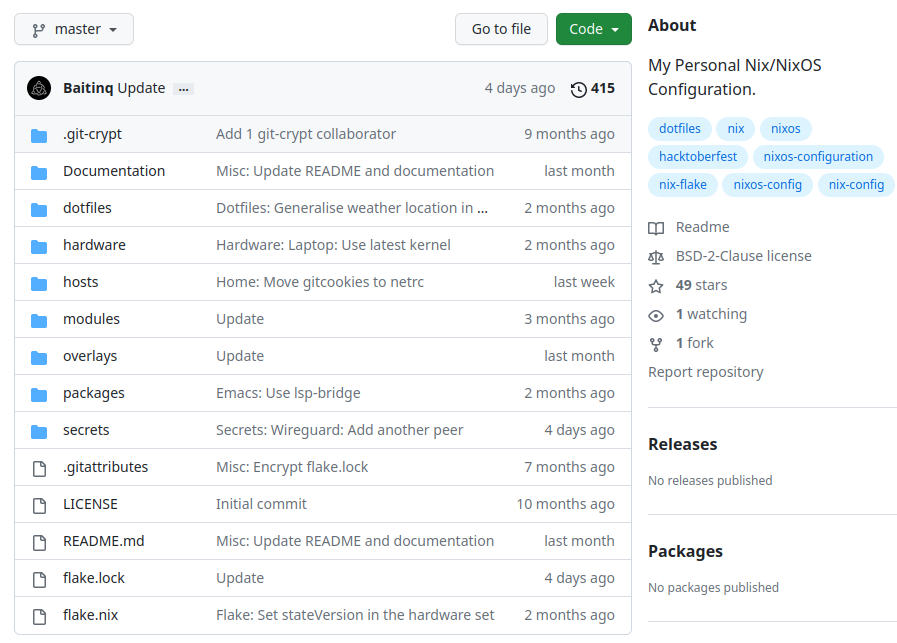
\includegraphics[scale=0.34]{img/20230413_10h27m54s_grim.png}
\end{frame}

\begin{frame}[fragile]
\frametitle{Configuracion minima de NixOS}
\begin{block}{configuration.nix}
\begin{verbatim}
{
    boot.loader.grub.device = "/dev/sda";

    fileSystems."/".device = "/dev/sda1";

    services.sshd.enable = true;
}
\end{verbatim}
\end{block}
\begin{block}{}
\begin{verbatim}
$ nixos-rebuild switch -I nixos-config=configuration.nix
$ nixos-rebuild switch --rollback
$ nixos-rebuild test -I nixos-config=configuration.nix
$ nixos-rebuild build-vm -I nixos-config=configuration.nix
\end{verbatim}
\end{block}
\end{frame}

\begin{frame}[fragile]
\frametitle{Configuraciones NixOS}
\begin{block}{configuration.nix}
\fontsize{9}{11}\begin{verbatim}
{ config, pkgs, ...} :
{
     imports = [ ./hardware.nix ];

     environment.systemPackages = with pkgs; [ thunderbird firefox vim ];
     
     users.users."alice" = {
       isNormalUser = true;
       home = "/home/alice";
       extraGroups = [ "wheel" "networkmanager" ];
    };

     services.xserver = {
       windowManager.i3.enable = true;
       displayManager.sddm.enable = true;
       videoDrivers = [ "nvidia" ];
     };

     networking.firewall.enable = true;
}
\end{verbatim}
\end{block}
\end{frame}

\begin{frame}
    \frametitle{El futuro de Linux}
    \begin{itemize}
        \item NixOS tiene problemas
        \item Alternativas: 
        \begin{itemize}
        \item Fedora Silverblue?
        \item Seguir como estamos?
        \end{itemize}
    \end{itemize}
    \begin{center}
            
\includegraphics[scale=0.34]{img/1366_2000.jpg}
    \end{center}
\end{frame}

\begin{frame}
\frametitle{Mas informacion}
\begin{center}
\begin{itemize}
    \item \begin{center}NixOS modules\end{center}
    \item \begin{center}Overriding\end{center}
    \item \begin{center}Flakes\end{center}
    \item \begin{center}Etc..\end{center}
\end{itemize}
\end{center}
\begin{columns}
        \column{0.6\textwidth}
\begin{itemize}
    \item \href{https://nixos.org}{NixOS website}
    \item  \href{https://nixos.org/manual/nixos/stable/}{Nix Manuals}
    \item  \href{https://nixos.org/guides/nix-pills/}{\textbf{Nix Pills}}
    \item  \href{https://learnxinyminutes.com/docs/nix/}{Learn X in Y minutes, where X=nix}
\end{itemize}
        \column{0.4\textwidth}
            
\includegraphics[scale=0.4]{img/207px-Home-nixos-logo.png}
\end{columns}
\end{frame}

\begin{frame}
    \frametitle{Gracias por escuchar!}
    \begin{center}
            
\includegraphics[scale=0.4]{img/207px-Home-nixos-logo.png}
            \begin{itemize}
                \item Preguntas
                \item Feedback
            \end{itemize}
    \end{center}
    \vspace{44}
    \href{https://github.com/Baitinq/nixos-config}{https://github.com/Baitinq/nixos-config}
\end{frame}


\end{document}
